\documentclass[12pt]{article}
\usepackage[a4paper, margin=0.8in]{geometry}
\pdfpagewidth 8.5in
\pdfpageheight 11.0in
\textheight 9.7in
\usepackage{color} %used for font color
\usepackage{amssymb, amsmath, multirow, commath, inputenc, titling, epic, paralist, graphicx, algorithm,algorithmic, tikz, xcolor,colortbl, environ, quoting, ragged2e, lipsum, caption}
\DeclareGraphicsExtensions{.pdf,.png,.jpg}
\DeclareGraphicsRule{.tif}{png}{.png}{`convert #1 `dirname #1`/`basename #1 .tif`.png}

\usepackage{sectsty}
\usepackage{multicol}
\sectionfont{\large}

\setlength{\droptitle}{-5.5em}
\setlength{\parindent}{30pt}

\begin{document}

\title{{\bf \large Utilizing an AI Approach to Pathfinding in Super Mario}\vspace{-2ex}}
\author{{\small Nick De Tullio, Michael Jalkio, \& Thomas Gautier}
\\ {\small nrd24@cornell.edu, mrj77@cornell.edu, tng26@cornell.edu}\vspace{-9ex}}
\date{}

\maketitle
\vspace{-7.5ex}
\begin{center}
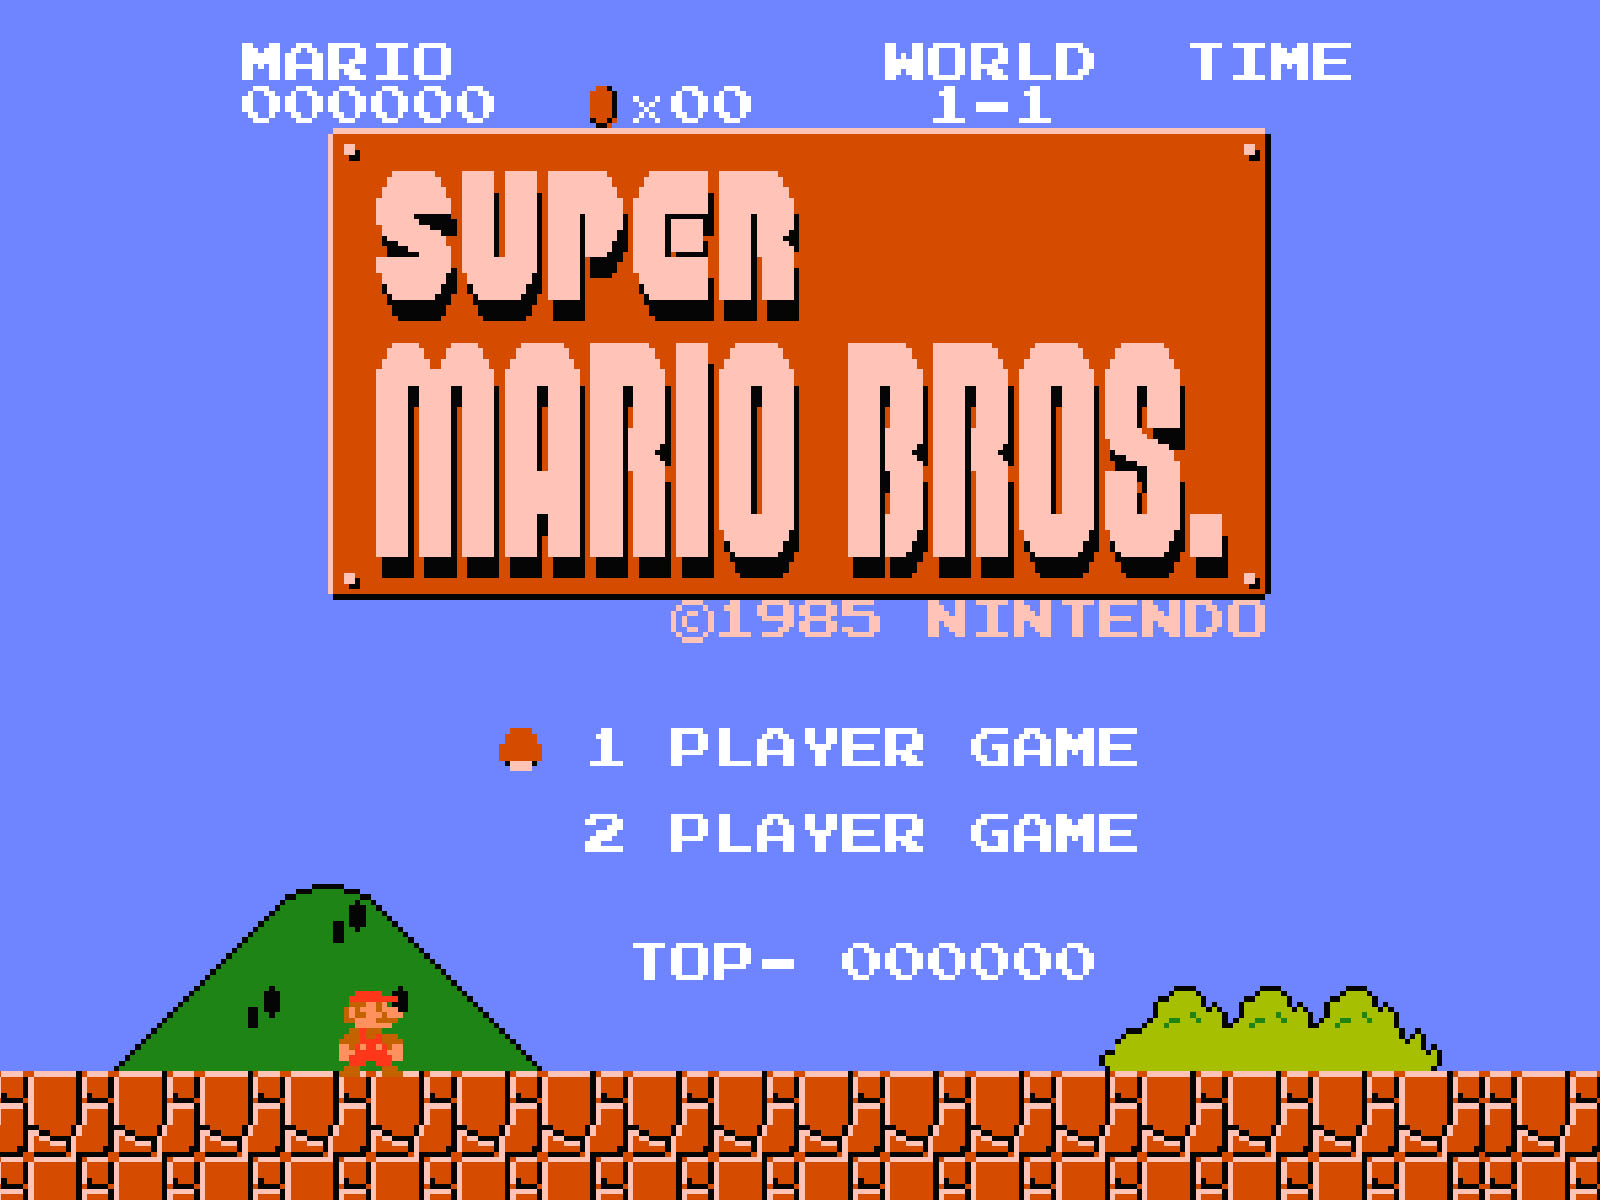
\includegraphics[width=0.65\textwidth]{waste_of_space} 
\end{center}
\vspace{-4.5ex}

\section * {Abstract}
This paper utilizes the Mario AI benchmark, to describe the success of both previously implemented Mario bots 
compared to our own implementation. The Mario AI Benchmark was introduced for use first in the IEEE Games 
Innovation Conference (ICE-GIC) and then later in Computational Intelligence Games (CIG) as a benchmark for 
reinforcement learning algorithms and other game AI techniques in a public domain clone of the platform game {\it 
Super Mario Bros}. Each year the CIG conducts a Mario AI Competition, in which they compare contestants 
submitted Mario bots to this benchmark. The goal of this paper is to determine the success of bots that were already 
created for this competition and then to decide whether an improved bot can be created. The bots that will be 
evaluated fell into three categories in the competitions A*-based, learning-based, and rule-based implementations.

\setlength{\columnsep}{.65cm}
\begin{multicols}{2}
\section * {Introduction}
A platform game, or platformer, is a video game which involves guiding an avatar to jump between suspended 
platforms, over obstacles, or both in order to advance the game. These challenges are known as jumping puzzles 
or freerunning. It is the job of the player to control the jumps in order to avoid letting their avatar fall from the 
platforms or miss the necessary jumps. The most common element of the genre of platform games is the jump 
button. Platform games originated in the early 1980s in side scrolling or 2D video games, which were eventually 
followed by 3D successors in the mid-1990s.

Super Mario Bros is a series of platform video games created by Nintendo, featuring the main character Mario who 
serves as the player's avatar. The game follows Mario's adventures in the fictional Mushroom Kingdom, where he 
runs and jumps across platforms and atop enemies in themed levels. In the game it is necessary for Mario to jump 
over enemies and between platforms. It is also beneficial to Mario to jump on enemies in order to prevent them 
from coming across his path again, provided that they do not have spiked turtle shells. Aside from staying alive and 
progressing towards the finish line, it is also beneficial to the player's score for Mario to collect coins by jumping 
into them as they are found in the level, as well as by jumping into bricks for coins that may be hidden. There are 
also a multitude of power-ups and items which give Mario special powers such as fireball-throwing, size-changing, 
and extra lives, which can also be found by jumping into bricks.

In order to make the benchmark possible the game was modified via the construction of an API that enabled it to be 
easily interfaced with learning algorithms and the various competitors' controllers. The modifications included the 
removal of the dependency on the system clock so that the learning algorithm can ``step" forward, removing the 
dependency on the graphical output, and substantial refactoring. Each step in the game corresponds to 40 
milliseconds of simulated time which has an update frequency of 25 frames per second. At each step, the controller 
receives a description of the environment, and outputs an action. The software that makes these modifications 
possible is a single threaded Java application, which allows for the key methods that a controller needs to 
implement to be specified in a single Java interface file.

There are many features that make \textit {Super Mario Bros} or platformers in general particularly interesting from 
an artificial intelligence or reinforcement learning perspective. What is likely the most important feature of the game 
is its potentially very rich and high-dimensional environment representation. When a human player views the 
game, he views a small part of the current level in two dimensions, with the screen centered on Mario. There are 
very rarely sparse views, in most cases there are dozens of objects such as brick blocks, enemies and collectable 
items. The static environment, such as grass, pipes, and brick blocks are laid out in a grid that covers 
approximately $19 * 19$ cells.

The entries for the 2009 Mario AI competition were classified into three broad categories, hard-coded heuristic, 
learning-based, and A*-based controllers. Hard-coded heuristics were the largest category, comprised of seven 
different controllers which were hand-constructed, non-adaptive, and did not use search-based methods for action 
selection. Learning based controllers were the second largest category comprised of two subcategories artificial 
evolution. There were three entries, the first used expression trees commonly used in genetic programming, the 
second evolved code for a stack-based virtual machine, and the third evolved a rule-based controller. The A*-based 
controllers were the most successful entries in the competition, beating the other controllers by a huge margin.

The success of the A*-based controllers over all other categories was considered by those running the competition 
to be a shortcoming, so in the 2010 Mario AI competition the level generator was expanded to include the possibility 
of generating dead ends. A dead end is defined as a situation where the player can choose one of two paths when 
moving forward, but at least one of the paths is blocked. This requires the player to backtrack and choose another 
path. Additionally, a number of other changes were made to the level generator in order to create harder levels. 
Some of the features introduced included greater control over numbers of items, the possibility of hidden blocks, and 
longer gaps. The difficulty was also increased for the hardest levels and some were literally impossible to finish. This 
allowed for the behaviors of various controllers to be tested in this difficult environment.

The 2010 championship allowed for both new and old competitors to enter, and there was a vast improvement in scores compared to the previous year. Given the changes to the level generator, the second competition allowed for controllers that were not exclusively A*-based to be successful. The 2010 competition consisted of four separate tracks in order to allow for different AI approaches to be more appropriately tested. The \textit {Gameplay track} was the direct continuation of the 2009 Mario AI Competition. In this track the goal for the submitted controllers was to clear as many levels as possible, with the exact same rules. 

The other tracks were the \textit {Learning track}, the \textit {Turing Test track}, and the \textit {Level Generation track}. The \textit {Learning track} was created to better test learning agents, by disadvantaging agents that did not incorporate any learning (online or offline). In this track the agents are tested on level that are unseen during the agent's development, but it is allowed to train on the track 10,000 times. It is only on the $10,001^{th}$ playthrough that the agent is scored. The \textit {Turing Test track} responded to the perceived machinelike quality of the 2009 entries, by asking competitors to submit controllers that behaved in a human-like fashion. This was done by showing non-expert humans both human and agent players and having them vote on whether the player was human or machine. The \textit {Level Generation track} used the Mario AI benchmark software for a content generation competition. Competitors were asked to submit personalized level generators that could produce new, playable levels that were significantly better than the levels generated in the previous years. The level generators were assessed by having humans play a test track followed by levels generated online for them by two level generators, choosing which was the most engaging.

The winner of the CIG 2010 Mario AI competition, which tested both the \textit {Gameplay track}, the \textit {Learning track}, and the \textit {Level generation track}, was the \textit{REALM} agent, which was built on a set of rules, which were evolved offline to maximize the distance travelled. The consequences of the evolved rules were high level plans which were executed with the help of A* planning.

\section * {Environment and State Space}
As stated above, the environment was based on Markus Persson's \textit{Infinite Mario Bros} which is an online,
public domain clone of Nintendo's classic \textit{Super Mario Bros} with open-source Java code. \textit{Infinite Mario Bros}
was primarily designed to be human-playable as an entertaining game, so many of the features of the source were incompatible 
or inconvenient for AI integration. Therefore, Karakovskiy et al. edited the \textit{Infinite Mario Bros} source to include an 
API that allowed interfacing with AI code, removing dependency on graphics output and the system clock to allow simulations 
to be run computationally and not graphically, with a temporal step size in simulated time of 40ms (25 Hz). 
The source was also extensively modified to include a more sophisticated level-generation class which allowed for both 
more complex levels than were available before and the ability to recreate levels using each level's seed. Karakovskiy et al. 
also added a significant number of parameters for level design that allowed programmers to specify certain aspects of each level, 
such as an enemy mask which determined the presence of various types of enemies, difficulty, length, and the frequency of dead 
ends that require backtracking (dead ends were not originally included in \textit{Infinite Mario Bros}). Their final software resulted in a 
cross-platform Java program that ran on a single thread and had low computation times for standard desktop machines of the time 
(they quote an estimate of order 10 levels per second on a 2009 MacBook with most of the computation time being used by the 
agents and not by the game simulation software).

The API consisted of two main interfaces and a ``Task" analysis interface. The benchmark software provides the environment interface 
to the AI which includes all the information available to it in-game. The environment is classified in a $22 * 22$ ``block" grid, with each block 
taking up a significant amount of pixel space. In each block, there were binary fields for passible/impassible terrain and for the presence of enemies. 
Because block coordinates were far too inaccurate for sufficient path calculations, the designers implemented exact (pixel space) coordinates for 
enemies in order to allow AI consoles the accuracy of human perception. Zoom levels were introduced that give the AI more detailed information about the 
state space, including levels of detail that distinguish all necessary details but don't distinguish between functionally equivalent enemies (for instance, enemies that 
can be killed by fireballs and can be jumped on are all classified the same) and a full zoom level that gives the AI the level of detail that the engine has access to.
Finally, the environment interface contained information about Mario's current state, including his mode (small, big, or fire), if he is on the ground, if he can jump, 
and if he is carrying a Koopa shell. Functionality for processing a raw bitmap image of the screen at each discrete time step was implemented but was not used by any AI routine.

The agent interface was to be implemented with the AI source code and controlled mario in each game. In order to understand the functionality of this interface we 
must first discuss the functionality of Mario himself. The original Nintendo had six inputs: four directional inputs and two miscellaneous buttons, A and B. 
In \textit{Super Mario Bros} and consequently in \textit{Infinite Mario Bros}, the ``up" button on the directional pad was not used and its intuitive functionality, 
the ``jump" command, was assigned to one of the two miscellaneous buttons. The other miscellaneous button was used to activate sprint and fire a fireball 
when Mario was in fire mode. The left and right directions on the directional pad move Mario left and right respectively, and the down button on the directional 
pad makes him crouch down. 

The agent interface calls the method \textit{getAction} at every discrete time step, in the case of simulated time every 40ms. 
The method takes an environment as input (the current game environment) and returns a  five-bit array of actions, one for each of the 
five used buttons as ``pressed" or ``not pressed". Buttons may be pressed simultaneously pressed, so there are therefore \(2^5 = 32\) 
actions that may be taken by the agent. While several of the elements in action space are pointless, not used, or rarely used (such as 
``left" and ``right" simultaneously which is meaningless, or ``jump" and ``crouch" which is a discrete action but rarely used). 

The combination of random level generation with certain complexities (such as dead ends that cannot be distinguished from regular levels upon 
entering but eventually requiring backtracking), the massive environment state space, and the relatively large action space makes for a very interesting 
AI problem that, as we will see, is not easily solved by pure computation. Rather, there are certain strategies that maximize survival and point collecting that are not
 quickly or effectively learned by learning agents and can be somewhat easily integrated into heuristic or rule-based algorithms.
 
\section * {Analysis of Agents}
We analyzed six different agents for this paper.  The first is the basic ForwardJumpingAgent which 
was a sample agent provided by the benchmark.  Three of the agents are the best agents within
their respective categories that were submitted 
for the CIG iteration of the competition.  There's one A* agent, one hard-coded rule based agent, and 
one learning agent.  Finally, we looked at two agents that we created.  The first was an attempt at a 
small improvement to the ForwardJumpingAgent that would jump out of holes when it fell in.  
The second was our own very simple rule based agent.

The analysis consisted of running the agents on 40 different levels.  They played 10 levels each 
on difficulties 0, 3, 5, and 10.  Each level within the set of 10 was progressively longer.  We analyzed 
the agents both quantitatively and qualitatively.  The quantitative analysis was the scoring system 
used in the competition.  It put the largest emphasis on the distance traveled, but also considers 
kills, Mario's mode (fire, large, small), time taken, and number of levels completed.  The qualitative 
analysis was simply watching the algorithms run through the levels and seeing if we could identify 
situations that they do not perform well in.  A table of our quantitative results is below:
\end{multicols}

\begin{center}
\begin{table}[h]
\resizebox{\textwidth}{!}{ 
\begin{tabular}{|c|c|c|c|c|c|c|c|c|c|c|}
\hline
Controller & D0      & D3      & D5      & D10     & Score   & Total Kills & Status & Time Left & Mode & Total \\ \hline
FJ         & 10660.2 & 2170.2  & 1994.2  & 1137.4  & 15962.0 & 71          & 9            & 6611      & 32         &     22685.0      \\ \hline
FJ2        & 8186.2  & 1859.1  & 1605.3  & 1158.7  & 12809.3 & 60          & 8            & 6470      & 31         & 19378.3   \\ \hline
GP         & 11108.5 & 2404.5  & 1397.9  & 1024.2  & 15935.2 & 99          & 10           & 6009      & 46         & 22099.2   \\ \hline
RB         & 11369.9 & 6555.2  & 3130.2  & 3291.9  & 24347.2 & 228         & 12           & 4968      & 19         & 29574.2   \\ \hline
A*         & 11628.8 & 11611.2 & 11651.2 & 11619.2 & 46510.4 & 414         & 40           & 4730      & 80         & 51774.4   \\ \hline
Amazing    & 11267.4 & 3103.8  & 2742.0  & 1199.3  & 18312.6 & 83          & 10           & 6035      & 21         & 24461.6   \\ \hline
\end{tabular}
}
\caption*{\footnotesize Controller Scores}
\end{table}

\vspace{-3ex}
\textsc{\scriptsize Results of our run of the various bots against our own controller titled amazing agent. explanation 
of column labels: fj: forward jumping, gp: genetic programming, rb: rule-base, A*: a-star search, amazing: our 
implemented agent (amazing agent), D0...D5: score at difficulty 0...5 respectively based on progress, score: sum of 
all the difficulties, status: number of levels completed, time left: sum of time remaining after each level, mode: sum of 
abilities that mario has at the end of each level, total: total score based on progress, kills, and time taken (used to 
calculate winner)}
\end{center}

\begin{multicols*}{2}
We will analyze the agents in the order of their score from the worst to the best.
\subsection*{ForwardJumpingAgent2}
The goal of ForwardJumpingAgent2 was to solve a problem faced by the original 
ForwardJumpingAgent: falling into gaps.  In this version of Mario it is possible to jump off of walls, 
so in some situations when you're falling down a gap it's possible to jump within the gap and free 
yourself.

ForwardJumpingAgent2 always keeps track of Mario's position on the x-axis and if it stays in the 
same position for a short time (signifying that it might be stuck against a wall) it attempts to jump left.  
Then if it finds itself falling for a short time again it assumes that it's on the other wall and tries to jump 
right.  When it isn't falling into this pattern, ForwardJumpingAgent2 follows the same behavior as 
the normal ForwardJumpingAgent.

What we found when scoring this agent was that it actually performed worse than 
ForwardJumpingAgent.  It completed only 8 levels (ForwardJumpingAgent completed 9), and 
traveled a shorter distance on average at all difficulty levels other than the hardest difficulty.

There were two main issues with this agent.  The first problem was that we misjudged how 
jumping off walls could help an agent.  While the ForwardJumpingAgent fell into gaps a lot, 
it very rarely fell onto the far wall within a gap.  In fact, while watching ForwardJumpingAgent2 it was 
never able to save itself from a gap, so it failed at its main purpose.

The other issue was that jumping off walls actually hurt the agent in many cases.  The most common 
case was that the agent would fail to make it over a wall in the environment on its first try, would jump 
left, and then would have to try to jump over the wall again.  In at least one case that was observed the 
agent failed to ever make it over the wall, and fell into that loop until it timed out.  In other cases the 
agent was hit by a bullet that was able to catch up to it, the agent jumped into an enemy that it had 
already passed, and the agent even jumped into gaps that it had already passed.

Overall, this naive attempt at an improvement was a failure.  We discovered that making ``small'' 
improvements to an agent can be more difficult than expected.

\subsection*{Genetic Programming Agent}
The second worst agent was a genetic programming agent created by Matthew Erickson.  
The agent used function detectors which were written by him, and the terminal nodes are a 
collection of four values.  The four values say whether the agent should go left or right, 
press jump or not, and press down or not.  He used a population of size 500 with 90\% 
crossbreeding, 9\% cloning and 1\% mutation.

The agent managed to complete 10 levels, which was better than either of the forward jumping 
agents.  However, it had very poor performance when the difficulty was 5 and 10.  Overall, it only 
did slightly worse than FowardJumpingAgent.

Watching the agent, the most interesting difference it has when compared to the other agents is 
that it quickly pushes all of the buttons on and off.  This gives the impression that while evolving 
the genetic program that there weren't many dominant ways to play.  Generally though, the agent 
simply moves forward and jumps.  It does appear to do a better job at killing enemies with both 
fire and by jumping at them.  It has also learned to wait for the piranha plants when they are outside 
of their pipes.

The main issue faced by this agent is the way that it quickly pushes all of the buttons.  This means that 
it never holds down the jump button, and can't jump over large walls or gaps.  Overall the agent 
doesn't seem to have to learned how to deal with gaps in the environment.  This is explainable, there 
are a large number of different gaps possible in Mario.  However, in most cases just jumping frequently 
works well.    Jumping kills enemies, gets over gaps, and allows you to traverse walls.  
The genetic program didn't have enough knowledge to assess why certain strategies 
worked and did not work in given situations, it just evaluated the fitness of different programs.  
Therefore, it only learned that jumping a lot was good.

The unfortunate truth of this agent was that it was the top performing learning agent in the competition 
we were assessing.  While to a human Mario is a simple game, there are many unique cases 
encountered that makes it a very hard game for an artificial intelligence agent to learn.

\subsection*{ForwardJumpingAgent}
This is the most simple agent (but beat two other agents in our set).  
All it does is run and jump whenever 
it can.  Surprisingly, this simple heuristic is enough to do fairly well on the benchmark and complete 
9 levels.  In the first iteration of the competition it came in 5th place out of 11 different agents.

What is interesting is how good this agent appears to a human observer.  Because the agent 
is able to jump at the soonest possible moment every time, it seems to be acting with a 
superhuman reaction time.  It does well because jumping in Mario is a very useful ability.  For 
most enemy types, jumping prevent Mario from being hit and also kill the enemy.  Jumping is the 
only way for Mario to traverse gaps.  It's also his only way to get over walls.  In the early levels that 
most of our agents are successful in, there are more safe spaces than danger zones, so just 
jumping quickly through the levels works.

Something that is noteworthy is ForwardJumpingAgent's lack of desire to acquire power ups.  There 
are many situations where this agent could have benefitted from waiting for a mushroom power up, or 
from backtracking and picking up a fire flower.  However, it always keeps running forward, and this 
sometimes leads it to die.

On the more difficult levels the spiny koopas become a major issue for ForwardJumpingAgent.  
Landing on top of these koopas hurts Mario, so jumping becomes worse.  There are also more gaps 
on the difficult levels for Mario to fall into.  Occasionally, Mario will have a moment of divine 
intervention where he dodges every gap, stomps a large number of enemies, and progresses far 
on a very difficult level.  However, this never lasts long enough to complete the longer levels.

ForwardJumpingAgent is a fantastic benchmark agent, and can certainly out-perform many 
human players of the game.  However, it isn't able to compete with the more sophisticated agents 
that were present in the competition.

\subsection*{AmazingAgent}
AmazingAgent is the rule-based agent that we created for this paper.  The idea was to start with 
ForwardJumpingAgent, find the situations that it failed the most frequently on, and then create 
an agent that would handle those cases more elegantly.  It did outperform ForwardJumpingAgent, 
completing one more level (for a total of 10 completed levels) and consistently traveled a further 
distance on all levels.  It was also a better killer than ForwardJumpingAgent, but that may have 
been a side-effect of progressing further.

There were a few things we disliked about ForwardJumpingAgent that we wanted to fix.  The 
first was that because it was always jumping, it would frequently jump into enemies that were above 
it.  The second was that it would jump into gaps in the environment.  The final thing was that always 
running right would sometimes cause the agent to run right into an enemy.  We thought that fixing these 
three major problems could lead to a big improvement.

AmazingAgent starts by getting the enemy observation data along with its own position.  If there is 
an enemy above and in front of Mario, it runs right without jumping.  If there is an enemy, it stops 
moving right and just jumps up (with the hope that it will land on top of the enemy).  Otherwise, 
it just runs and jumps in the same way as FowardJumpingAgent.

Unfortunately, we found that writing logic to avoid jumping in gaps was very difficult.  The main 
problem is that there are a number of corner cases that need to be handled.  The simple logic would 
be ``if you are at a jump's distance from a gap, run towards it.  Then jump once you are closer.''  
However, this doesn't always work.  For example, take the following situation:
\begin{center}
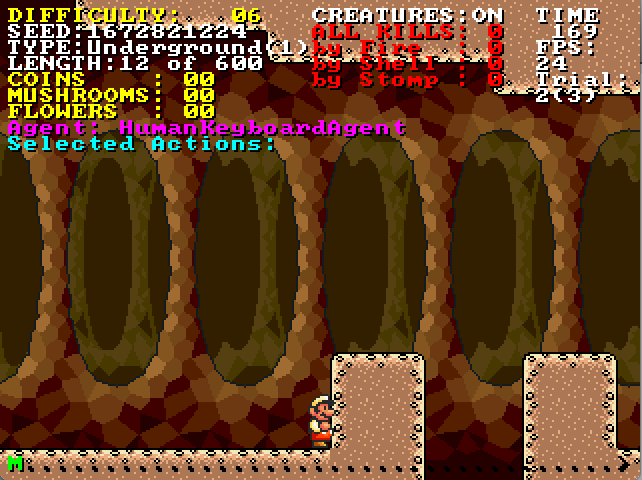
\includegraphics[scale=0.6]{gap_issue}
\end{center}
In this case, Mario is at a distance where jumping could lead him to jump into the gap.  However, 
he needs to jump in order to get on top of the wall.  There are a number of situations similar to 
this, and we ultimately abandoned the goal of having Mario avoid gaps.

Just avoiding enemies was enough to lead to an improvement for AmazingAgent.  This is most 
visible when Mario waits for piranha plants to retreat into their pipes before jumping past them.  
There was some strange behavior where Mario would refuse to jump past pipes because he believed 
the piranha plant was still a threat, but we resolved that by making Mario aware of his position.  If 
Mario stays in the same position on the x-axis for too long he jumps forward whether or not he believes 
it's safe.

The only downside to this agent is that sometimes not jumping when an enemy is above backfires.  
We observed multiple situations where waiting led Mario to be hit by a bullet which came from behind 
him.  There were other situations where Mario was waiting for an enemy on a ledge above him, and 
the enemy simple walked down and fell on top of Mario.

We were very satisfied with this agent, which would have come in fifth place out of twelve in the 
first iteration of the Mario AI competition.  It has very simple behavior, but sometimes that's the best 
that you can do in a complex game.

\subsection*{Ruled-Based Agent}
The second best agent was a rule-based agent created by Trond Ellingsen which he called 
LuckyAgent.  What is most amazing to us about this agent is how succinct its implementation is.  
In the ICE-CIG competition the top rule-based agent was created by Sergio Lopez, and was over 
1000 lines of code.  Ellingsen's agent is only 100 lines and manages to beat all agents outside of the 
A* solutions.  The fact that the logic and strategy for a game as complex as Mario can be captured 
in only 100 lines is an impressive accomplishment.

LuckyAgent's methodology is to calculate what is nearby, and then to make appropriate jumps.  It takes 
into consideration Mario's speed, his distance from gaps or enemies, and whether or not he's 
currently jumping.  It also does some cool things such as always jumping the correct amount to 
get over a wall (so it makes small jumps to get up the stone steps that are frequent in the game).  
LuckyAgent is also a great killer because it always tries to time jumps so that it lands 
on top of enemies.  It only beats two levels more than the AmazingAgent, but defeats almost three 
times as many enemies in that time.  Although it can't beat the harder levels, it gets consistently further 
than the lower ranked agents.

When you watch LuckyAgent it does some interesting things that no other agents do.  For example, 
unless it sees an enemy or gap in the distance it will wait until it runs into a wall to jump over it.  
It also sometimes slows down before a gap and waits until it's close to jump over it.  This makes it 
appear to play levels more ``safely'' than the other agents in the competition.  It also never breaks 
bricks which is interesting, it doesn't seem to think they're worthy of jumps.  Similar to the other agents, 
it does not go after power ups which seems like an oversight.  The most impressive thing that 
LuckyAgent does is jump on pipes when the piranha plant is also on it.  It jumps just barely onto the 
edge so it's not touching the piranha plant, and will then jump up and over it.

The agent faces many of the same issues as other agents.  Bullets from behind sneak up on it.  It 
will also sometimes wait under a ledge and let an enemy fall on top of itself.  LuckyAgent doesn't seem 
to differentiate between spiny koopas and regular koopas and goombas, so it will jump on top of them.  
This agent is impressive, but perhaps it would benefit from some additional logic.

\subsection*{A* Agent}

\end{multicols*}

\end{document}
